\section{实验结果和分析}

本节中,我们会依次分析实验结果并回答上述提出的三个研究问题。

\subsection{有效性}

我们首先实验评估\wa 在单元格聚类和缺陷检测方面的有效性,然后和其他五个电子表格缺陷检测技术的结果进行比较。

\begin{table}[tbp]
    \centering
    \caption{6个电子表格缺陷检测技术的检测结果}
    \label{table2}
    \large
    \resizebox{\columnwidth}{!}{
    \begin{tabular}{|c|c|c|c|c|c|c|}
    \hline
    \textbf{技术} & \textbf{检测出} & \textbf{TP} & \textbf{FP} & \textbf{$precision_d$} & \textbf{$recall_d$} & \textbf{$F\text{-}measure_d$} \\
    \hline
        UCheck & 204 & 1 & 203 & 0.5\% & 0.1\% & 0.00 \\
    \hline
        Dimension & 1,824 & 14 & 1,828 & 0.8\% & 0.7\% & 0.01 \\
    \hline
        AmCheck & 2,372 & 1,316 & 1,030 & 56.1\% & 66.7\% & 0.61 \\
    \hline
        CACheck & 1,866 & 1,350 & 516 & 72.3\% & 68.4\% & 0.70 \\
    \hline
        CUSTODES & 2,380 & 1,539 & 841 & 64.7\% & 78.2\% & 0.71 \\
    \hline
        WARDER & 1,612 & 1,415 & 197 & 87.8\% & 71.9\% & 0.79 \\
    \hline
    \end{tabular}}
\end{table}

就缺陷检测而言,表~\ref{table2}对比了所有6个检测技术的结果,包括精度,召回率,\fmd,检测出的缺陷数量,以及其中包含的真阳性和假阳性。从表中,我们观察到:

\begin{enumerate}
    \item 由于他们有限的分析范围,\uc 和\di 获得了较低的分数(精度和召回率都低于1\%,\fmd 值也仅有0.01),这点也与之前的实证研究结果~\cite{zhang2017effectively}保持一致;
    \item 由于他们有效的分析模式(比如,单元格元组),\am 和 \ca 获得了较好的分数(56.1-72.3\%的精度,66.7-68.4\%的召回率,以及0.61-0.70的\fmd 值);
    \item \cu 比 \ca 获得了略微更好地分数(0.71的\fmd 值),以及对召回率的较大提升(72.8\%,对应的\ca 召回率为68.4\%);
    \item 如同预期的那样,\wa 关注于提升检测精度,对比于\cu 获得了大幅度提升,从64.7\% 提升到 87.8\%,最终总体上提升了\fmd 的值,从0.71到0.79,尽管对召回率有6\%的牺牲。 从数据中,可能产生一定疑惑:\cu 比 \wa 多检测出124个真阳性,但同时伴随着更多的假阳性(达644个),这对于终端用户的人工验证来说是很大的负担。
\end{enumerate}

\begin{figure}%
    \centering
    \subfloat[精度比较(仅展示被影响的工作表)]{{
        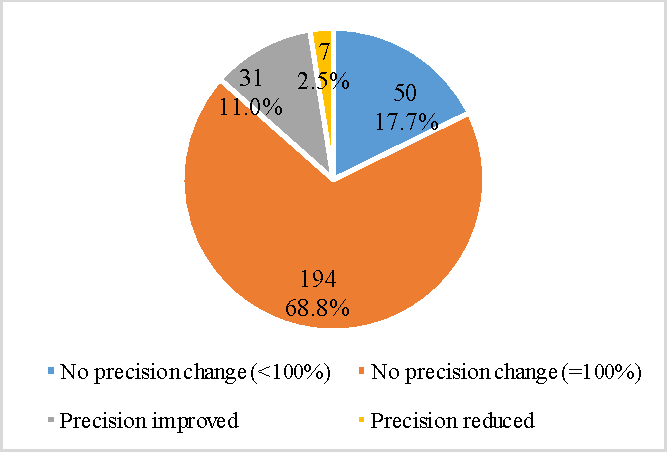
\includegraphics[width=0.40\textwidth]{figure/figure5a.pdf} 
        \label{figure5a}
        }}%
    \subfloat[召回率比较(整体)]{{
        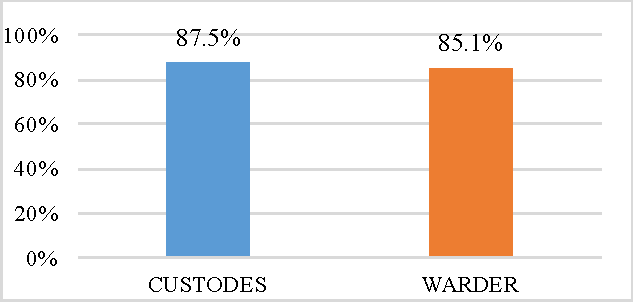
\includegraphics[width=0.55\textwidth]{figure/figure5b.pdf} 
        \label{figure5b}
        }}%
    \caption{CUSTODES 和 WARDER 的单元格聚类结果}%
    \label{figure5}%
\end{figure}

就单元格聚类而言,图\ref{figure5}比较了\cu 和 \wa 在精度和召回率两方面的结果。从精度比较来看(如图\ref{figure5}(a)),我们把包含至少有一个单元格类的282个工作表分成两类:
\begin{enumerate}
    \item \wa 提升了其中31个工作表的精度,降低了7个;
    \item 对于余下精度保持不变的244个工作表,其中194个已达到100\%(即上限)。
\end{enumerate}
换言之,\wa 提升了225个工作表的单元格聚类精度,要么是实际提升精度,要么已经达到上限。如图\ref{figure6}所示,我们进一步观察这38个精度产生变化的工作表。我们不难发现,\wa 在不同程度上提升了单元格聚类的精度(0.3\%-94.6\%,平均20.7\%),这样的精度提升是显著的,远多于精度受损的部分。另外从图\ref{figure5}(b)中,我们也注意到,\wa 在精度提升上的有效性也仅导致召回率的轻微下降(2.4\%)。

\begin{figure*}
    \centering
    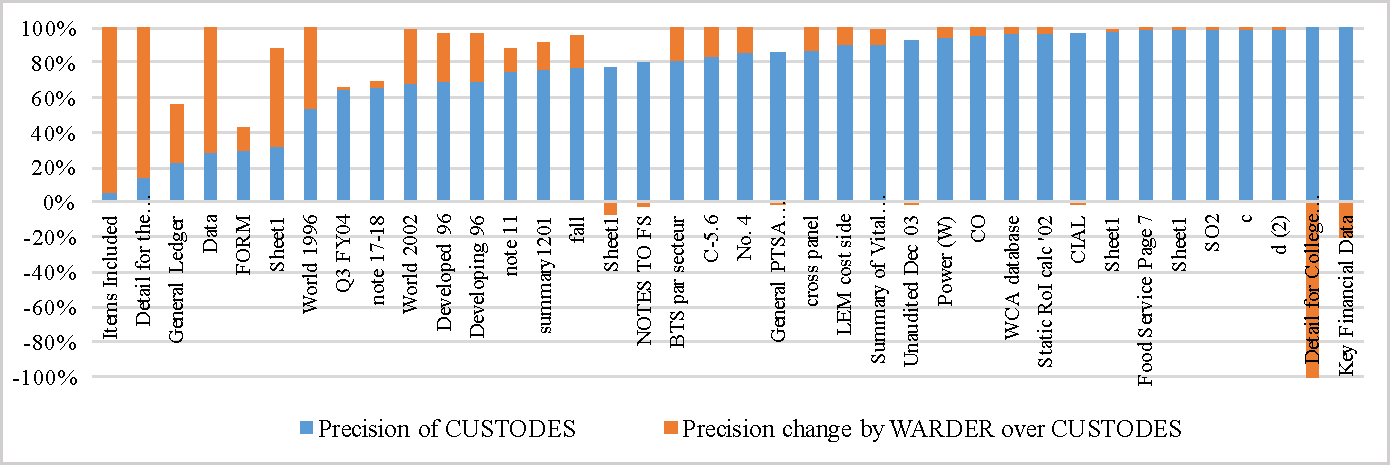
\includegraphics[width = \columnwidth]{figure/figure6.pdf}
    \caption{CUSTODES 和 WARDER 的单元格聚类结果(精度变化方面)}
    \label{figure6}
\end{figure*}
\begin{figure}[tp]
    \centering
    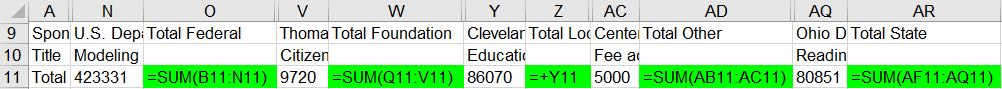
\includegraphics[width = \columnwidth]{figure/figure7.jpeg}
    \caption{工作表“Detail for College of Education” (包含一个绿色标记的单元格类)}
    \label{figure7}
\end{figure}

如图~\ref{figure6}所示,我们也观察到,\wa 对大多数精度受影响的工作表是正面作用,但也有极少量的例外情况,如名为“Detail for College ...”的工作表,它的聚类精度从100\%降低到了0。因此,我们进一步检查了该工作表的聚类情况。如图\ref{figure7}所示,人工标记的结果是,{O11,W11,Z11,AD11,AR11}应该被安排在同一个类中。\cu 看似正确地对这些单元格进行了分类,而\wa 分类得很差。然而,我们发现这五个单元格实际上包含不同的公式,因此它们违反了\wa 的 \wcvp (在这些单元格中不存在一个公共的计算语义能够覆盖过半数量)。事实上,这个单元格类的确不包含任何缺陷。因此,这个单元格聚类精度下降的案例并不影响\wa 的缺陷检测能力。

因此,针对研究问题1,我们能够得出如下结论:\textit{\wa 在单元格聚类和缺陷检测方面是有效的。它极大地提升了精度,达15.5-87.3\%,并且在所有被比较的电子表格缺陷检测技术中,取得了最佳的 \fmd 值(0.79)。}

\subsection{相关性}

\begin{table}[tbp]
    \centering
    \caption{\wa 相对于 \cu 在单元格聚类和缺陷检测上的的精度变化 ($\uparrow$: 精度提升, $\downarrow$: 精度下降, $\to$: 精度保持不变)}
    \label{table3}
    %\Large
    \begin{tabular}{|m{.16\columnwidth}<{\centering}|m{.16\columnwidth}<{\centering}|m{.16\columnwidth}<{\centering}|m{.08\columnwidth}<{\centering}|m{.18\columnwidth}<{\centering}|}
    \hline
    \textbf{相关性类型} & \textbf{聚类的精度变化} & \textbf{缺陷检测的精度变化}  & \textbf{\# 工作表} & \textbf{总计} \\
    \hline
        \multirow{3}{1.2cm}{正相关} & $\uparrow$  & $\uparrow$ & 8 & \multirow{3}*{126 (90.0\%)}\\
    \cline{2-4}
        ~ & $\downarrow$ &  $\downarrow$  & 2 & ~\\
    \cline{2-4}
        ~ & $\to$ &  $\to$  & 116 & ~\\
    \hline
            \multirow{4}{1.2cm}{负相关}& $\uparrow$ &  $\to$  & 5  & ~\\
    \cline{2-4}
         ~ & $\uparrow$  & $\downarrow$ & 2 & \multirow{4}*{9 (6.4\%)}\\
     \cline{2-4}

        ~ & $\downarrow$ &  $\to$  & 2 & ~ \\
    \cline{2-4}
        ~ & $\downarrow$ &  $\uparrow$  & 0 & ~ \\
    \hline
    \multirow{2}*{不相关} & $\to$  & $\uparrow$ & 5 & \multirow{2}*{5 (3.6\%)}\\
    \cline{2-4}
        ~ & $\to$ &  $\downarrow$  & 0 & ~ \\
    \hline
    合计 & - & - & 140 & 140 (100.0\%) \\
    \hline
    \end{tabular}
\end{table}

在这一小节里,我们研究\wa 相对于 \cu 在单元格聚类和缺陷检测上的的精度提升。

如表\ref{table3}所示,我们用三个符号 $\uparrow$,$\downarrow$和$\to$分别表示精度提升,精度下降,以及精度保持不变这三种情况。按照相关性类型,我们把人工标记中至少含有1个缺陷的工作表分成3个类型:
\begin{enumerate}
    \item \textit{正相关}:当相对于\cu 的单元格聚类,\wa 的精度有提升,下降或不变时,在缺陷检测上精度变化表现一致;
    \item \textit{负相关}:当相对于\cu 的单元格聚类,\wa 的精度有提升时,在缺陷检测上精度下降或保持不变;或者相反地,\wa 的精度下降时,在缺陷检测上精度提升或保持不变;
    \item \textit{不相关}:其他的组合情况,均划归此类,既不表现出正相关,也不表现出负相关。
\end{enumerate}
总得来说,我们能够观察到:第一类占据主导(90\%),因此表明 \wa 对单元格聚类的精度提升方法的确能够带来缺陷检测精度的提升,并且九成比例成明显正相关。

\begin{figure}%
    \centering
    \subfloat[CUSTODES 和 WARDER 在单元格聚类上的精度]{{
        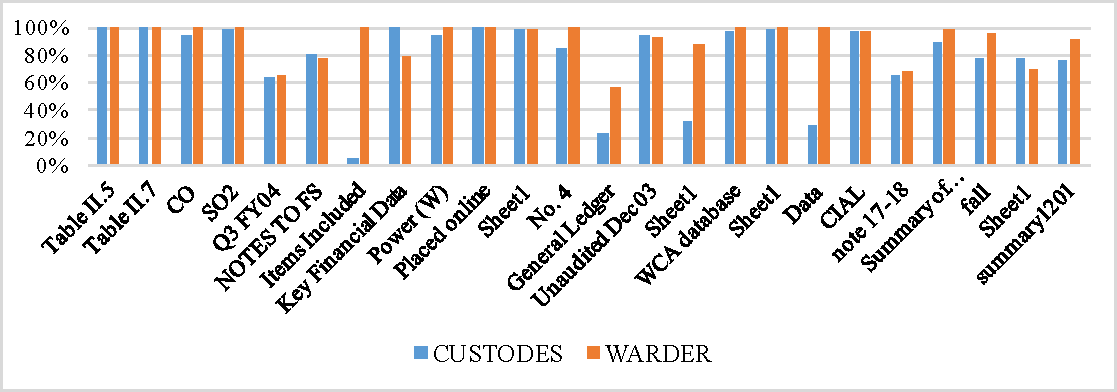
\includegraphics[width=.95\columnwidth]{figure/figure8a.pdf} 
        \label{fig8a}
        }}%
    \qquad
    \subfloat[CUSTODES 和 WARDER 在缺陷检测上的精度]{{
        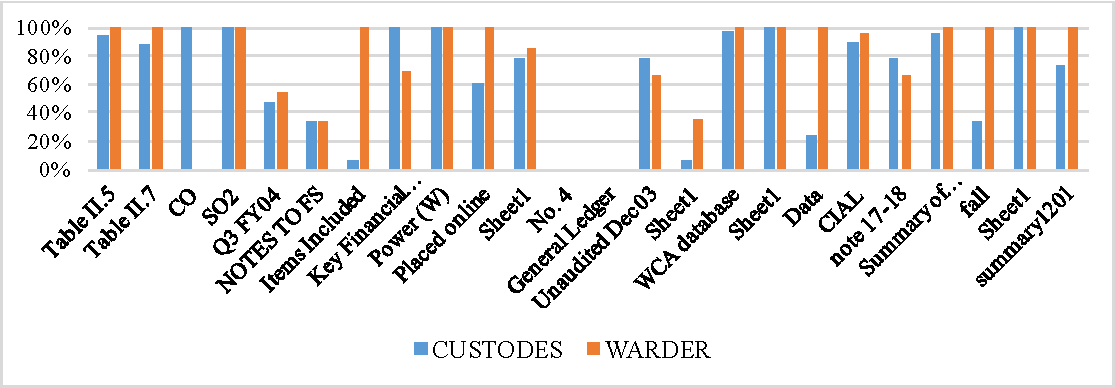
\includegraphics[width=.95\columnwidth]{figure/figure8b.pdf} 
        \label{fig8b}
        }}%
    \caption{\cu 和 \wa 中有精度变化的工作表}%
    \label{figure8}%
\end{figure}
\begin{figure}[tbp]
    \centering
    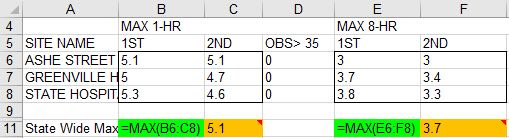
\includegraphics[width = .95\columnwidth]{figure/figure9.jpg}
    \caption{工作表 ``CO'' (两个类分别用绿色和橙色标记)}
    \label{figure9}
\end{figure}

图\ref{figure8}展示了在单元格聚类和缺陷检测上\wa 和 \cu 的更细致的精度对比。为了展示的清晰性和简洁性,我们移除了精度前后无变化的 116 个工作表,仅罗列出剩下的 24 个。细致的观察可以发现:在单元格聚类和缺陷检测的精度变化上大部分情况下是正相关的。不过,其中一个例外是名为“CO”的工作表,在这张表上,\wa 的缺陷检测精度从100\%跌至 0,然而单元格聚类精度却有提升。我们进一步检查了这个情况。如图\ref{figure9}所示,人工认为单元格{B11,E11}(绿色标记) 和{C11,F11}(橙色标记)应该构成两个类,并且单元格 C11 和 F11 应该是两个缺陷(用红色三角标记)。\cu 因为意外地将这四个单元格分成同类,而偶然地检测到了这两个缺陷。这是偶然的,因为这四个单元格本质上并不共享相同的计算语义(两个绿色的单元格用来计算最大值,而两个橙色的单元格用来计算第二大值)。\cu 只是简单地将两个橙色的单元格标记为缺陷,因为他们仅仅包含纯数值(丢失公式的缺陷)。另一方面,\wa 仅仅将{B11,E11}划分为同一类,因此无法检测到其中的任何缺陷。它漏掉了两个橙色单元格,因为它们不包含任何公式,且没有和它们相同计算语义的公式存在,因而无法被识别到任何类中。当没有额外的证据时(例如,更多的计算第二大值的单元格出现,并且相应的公式也存在于某些单元格中),\wa 选择不把这些单元格放到任何类中(否则,可能导致更多的假阳性)。

因此,针对研究问题2,我们能够得出如下结论:\textit{\wa 在单元格聚类上的改进的确进一步提升了缺陷检测的结果,这一相关性得到90.0\%的工作表的数据支撑。}


\subsection{独立性}

\begin{table}[tbp]
    \centering
    \caption{\cu 和 \wa 在不同配置下的缺陷检测结果}
    \label{table4}
    \large
    \resizebox{\columnwidth}{!}{
    \begin{tabular}{|c|c|c|c|c|c|c|}
    \hline
    \textbf{技术} & \textbf{检测出} & \textbf{TP} & \textbf{FP} & \textbf{$precision_d$} & \textbf{$recall_d$} & \textbf{$F\text{-}measure_d$} \\
    \hline
        CUSTODES & 2,380 & 1,539 & 841 & 64.7\% & 78.2\% & 0.71 \\
    \hline
        WARDER-sc &2,083 & 1,506 & 577 & 72.3\% & 76.3\% & 0.74\\
    \hline
        WARDER-mc &2,164 & 1,507 & 657 & 69.6\% & 76.3\% & 0.73\\
    \hline
        WARDER-wc &2,071 & 1,498 & 573 & 72.3\% & 75.9\% & 0.74\\
    \hline
        WARDER-full & 1,612 & 1,415 & 197 & 87.8\% & 71.9\% & 0.79 \\
    \hline
    \end{tabular}}
\end{table}

最后,我们研究\wa 的三个有效性精化在检测电子表格缺陷上各自的表现。\wa 被配置成单独使用每一种精化方法(正如前面提到的,命名为\wasc,\wamc 和\wawc ),并和同时使用三种方法的\wa 作比较(\wa -full)。

表\ref{table4}对比了\cu 和 \wa 的四种配置的缺陷检测结果。我们可以观察到:
\begin{enumerate}
    \item \wa 的每个有效性精化是有用的,并且各自能够比\cu 在缺陷检测精度上提升 4.9-7.6\%,在召回率上有较小的牺牲(1.9-2.3\%),最终对\fmd 值有小幅提升(从 0.71 提升到 0.73-0.74);
    \item 组合所有三种有效性精化(即\wa -full) 可以获得最高的精度(87.8\%)和\fmd 值(0.79),这也和之前的表\ref{table1}数据相吻合。
\end{enumerate}

因此,针对研究问题3,我们能够得出如下结论:\textit{\wa 的三个有效性属性能够各自独立展现出对缺陷检测的正面效果;同时在三者组合运用时,也能够获得整体的最佳效果。}